% !TEX program = xelatex
\documentclass{article}
\usepackage{/Users/jay/LaTeX/cs}
\usepackage{xeCJK}

\newcommand{\hmwkClass}{Probability and Statistics, Spring 2018}
\newcommand{\hmwkTitle}{Homework 3}
\newcommand{\hmwkDueDate}{April 24, 2018}
\newcommand{\tb}{\textbf}

\begin{document}

\thispagestyle{empty}
\section*{\hmwkClass \\
    \normalsize{\hmwkTitle} \\
    \normalsize{DUE DATE: \hmwkDueDate}
}

\hfill{B03902129 \, 資工四 \, 陳鵬宇}

\begin{enumerate}
    \item [\textbf{3.2.6}]

    To find the PMF of $Y$, we need to know the set of $Y$ first.

    It's easy to see that $Y = \{0, 1, 2\}$.

    $$
    \text P_Y(y) =
    \begin{cases}
        1 - p    & y = 0 \text{ (first goes out)}, \\
        p(1 - p) & y = 1 \text{ (first goes in, then second goes out)}, \\
        p^2      & y = 2 \text{ (first goes in, then second goes in)}, \\
        0        & \text{otherwise}.
    \end{cases}
    $$

    \item [\textbf{3.3.1}]

    \begin{enumerate}[label=(\alph*)]
        \item
        
        $$
        \text P_Y(y) =
        \begin{cases}
            1 / 11 & y = 5, 6, 7, \dots, 15, \\
            0      & \text{otherwise}.
        \end{cases}
        $$

        \item

        $$\text P[Y < 10] = \sum_{i = 5}^9 \text P_Y(i) = 5 / 11.$$

        \item 

        $$\text P[Y > 12] = \sum_{i = 13}^15 \text P_Y(i) = 3 / 11.$$

        \item

        $$\text P[8 \le Y \le 12] = \sum_{i = 8}^12 \text P_Y(i) = 5 / 11.$$

    \end{enumerate}

    \item [\textbf{3.4.6}]

    The CDF are

    $$
    \text F_Y(y) =
    \begin{cases}
        0       & y < 0, \\
        1 - p   & 0 \le y < 1, \\
        1 - p^2 & 1 \le y < 2, \\
        1       & y \ge 2.
    \end{cases}
    $$

    The plottings are

    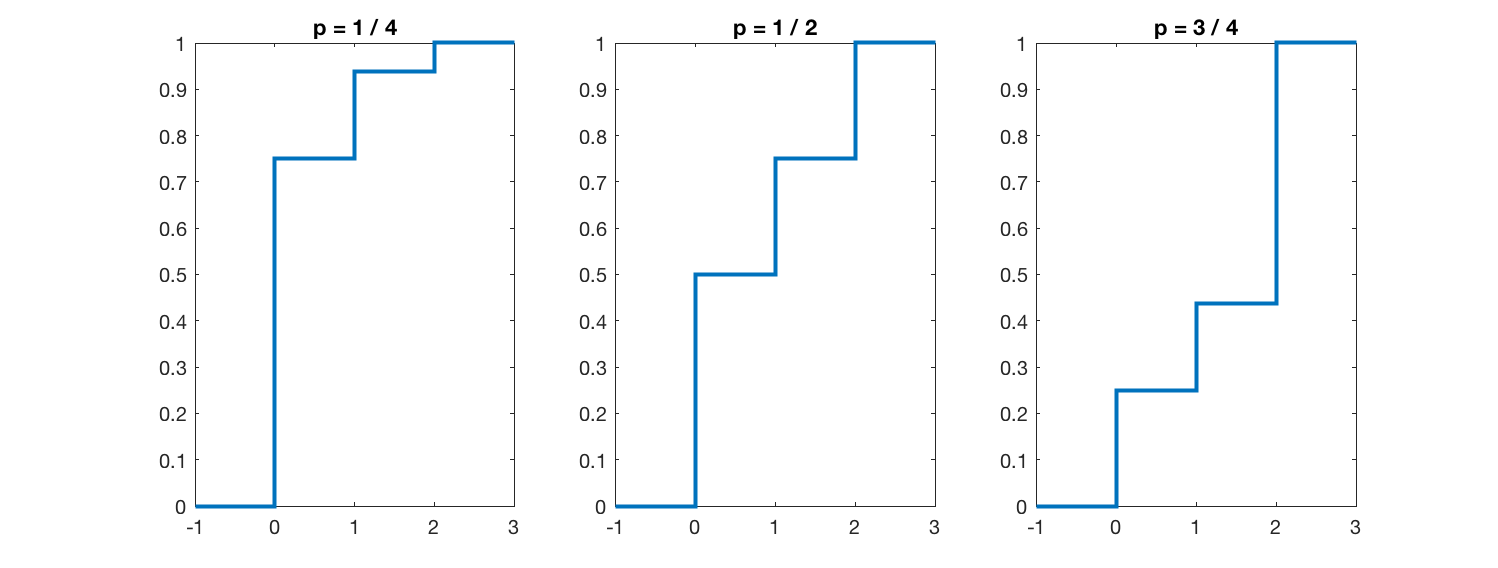
\includegraphics[width=0.8\textwidth]{img/3.4.6.png}

    \item [\textbf{3.5.10}]

    \begin{enumerate}[label=(\alph*)]
        \item

        $$
        \text P_R(r) =
        \begin{cases}
            1 - (\frac{1}{2})^{20} & r = 0, \\
            (\frac{1}{2})^{20}     & r = 20,000,000, \\
            0                      & \text{otherwise}.
        \end{cases}
        $$

        \item

        $$
        \text P_L(l) =
        \begin{cases}
            (\frac{1}{2})^{20}(1 - (\frac{1}{2})^{20})^{l - 1} & l = 1, 2, \ldots, \\
            0                & \text{otherwise}.
        \end{cases}
        $$

        \item The expected reward a customer earned

        $$E[R] = 20,000,000 \cdot (\frac{1}{2})^{20} \approx 19.07 < 20.$$

        The casino company should offer this game.


    \end{enumerate}

    \item [\textbf{3.6.2}]

    \begin{enumerate}[label=(\alph*)]
        \item 
        
        From 3.4.2, we have

        $$
        \text P_X(x) =
        \begin{cases}
            0.2 & x = -1, \\
            0.5 & x = 0, \\
            0.3 & x = 1, \\
            0   & \text{otherwise}.
        \end{cases}
        $$

        Therefore

        $$
        \text P_V(v) = \text P_{|X|}(v) =
        \begin{cases}
            0.5 & v = 0, \\
            0.5 & v = 1, \\
            0   & \text{otherwise}.
        \end{cases}
        $$

        \item 
        $$
        \text F_V(v) =
        \begin{cases}
            0   & v < 0, \\
            0.5 & 0 \le v < 1, \\
            1   & 1 \le v.  \\
        \end{cases}
        $$

        \item
        $$
        \text E[V] = 0 \cdot 0.5 + 1 \cdot 0.5 = 0.5.
        $$

    \end{enumerate}


\end{enumerate}

\end{document}